
\section{WORKBOOK LESSON 1
WORKBOOK AND CHART EXAMINATION}


\subsection{READING NORTH AND SOUTH INDIAN CHARTS}

 

The Vedic astrology course Workbook aims at providing the student a more practical orientation in reading charts. In this regard it follows the type of format that tutorial programs offer in greater detail. For students considering what a tutorial program may bring they can gain a taste of it through the Workbook.

 

The first two lessons of the Workbook are a good review and summary of important basic principles. The next several lessons provide more advanced chart analysis. The first four lessons of the Workbook follow Part I of the course. Lessons 5 and 6 follow Part II of the course. The final appendix chapters provide interesting advanced information on important issues in Vedic Astrology.

 

The Workbook emphasizes medical astrology along with basic astrology, following the same orientation as the course. All charts are done with the Lahiri Ayanamsha because that has become the standard adopted by the CVA. However we do explore the issue of Ayanamsha further in the appendix and do not mean that other Ayanamshas do not have their validity.

 

\subsubsection{Workbook Testing – Study Questions Only}
 

The Workbook contains Study Exercises and Study Questions but it has no Final Questions to return to the Institute as do the other three sections of the course. However some Final Questions at the end of Parts I and II of the course relate to the Workbook and require finishing it in order to answer them properly. Please make sure that you do these Study Exercises or you will not gain full benefit from this material.

 

The Workbook may cause more questions to arise in your minds. Please try to email or write these to us as it is not easy to be available by phone. Remember also that in the limitations of a correspondence course we cannot take on all possible questions or do chart interpretations outside of the course material. We appreciate your patience in the matter.

 

We hope that this new Workbook adds a helpful dimension to your study of Vedic Astrology and that it encourages you to do similar projects of our your own to help learn this profound subject.

 

Reading the Two Different Types of Vedic Charts (North Indian and South Indian)
North and South Indian Charts
While a Vedic astrologer may prefer either North or South Indian charts for personal usage, he or she should be able to read both fluently. Otherwise following books or teachers using the different systems will not be easy. Most Vedic astrologers today learn how to read both types of charts. Many important books on Vedic astrology, traditional or modern, may show only one type of charts by way of analysis.

 

In this lesson we will examine both types of charts and show you how to read each. Learning to read both is an excellent tool for studying Vedic Astrology because each shows certain aspects of the system more clearly than the other type of chart.

 

\subsection{The North Indian Chart and Examination of the Houses}
 

The North Indian chart is what I would call a “house chart” because in it the houses always remain the same, while the signs change depending upon the Ascendant. It is easier to see the role and value of different houses in the North Indian chart. Though I mainly use the South Indian chart myself, I usually use the North Indian as the house or bhava chart.

 

The North Indian chart can be initially confusing to people because it identifies the signs by numbers (which most people expect to indicate the houses), while the positions of the houses are understood. The numbers in the chart are always those of the signs, not of the houses. The numbers of the houses are not given because they follow a constant order. Hence if the number 4 is at the top of the chart it means Cancer Ascendant, if 11 Aquarius, and so on.

 

The top always represents the first house or Ascendant and the eastern direction. From it the other houses are counted off in a counter-clockwise direction. The fourth house is to the left, the seventh house at the bottom, and the tenth house to the right. With the first house at the top the chart shows how the individual, represented by the first house, rises or falls in life. The seventh house or relationship is his foundation. The tenth and fourth houses are like his right and left sides.

 

The main advantage of the North Indian chart is that house positions are clearly evident, particularly the angles. The angles – houses 1, 4, 7 and 10 – are the pillars of the chart. They hold up the chart like four pillars hold up a house.

 

Natural benefics in the angles give grace, fortune and happiness. On the other hand, natural malefics in the angles cause suffering, enmity, disease and misfortune. A simple glance at the North Indian chart shows these angular positions immediately, giving a clear insight into the basic strength or weakness of the chart.

 

In fact all house positions are easier to read from the North Indian chart. Once the student learns the position of other house divisions in the chart they will be easy to see at a glance.

 

However, the North Indian chart requires a Moon chart or Chandra Chakra to read houses from the Moon. Sometimes a Sun chart or Surya Chakra is added for reading houses from the Sun.

 

\subsubsection{Sample North Indian Chart}

 

Look at the sample chart done in the North Indian style. First use a pen and number the different houses starting with the first house at the top. Then memorize the house orientation of the North Indian chart so that you dont have to mark the houses by numbers again.

 \begin{figure}[h]
\centering
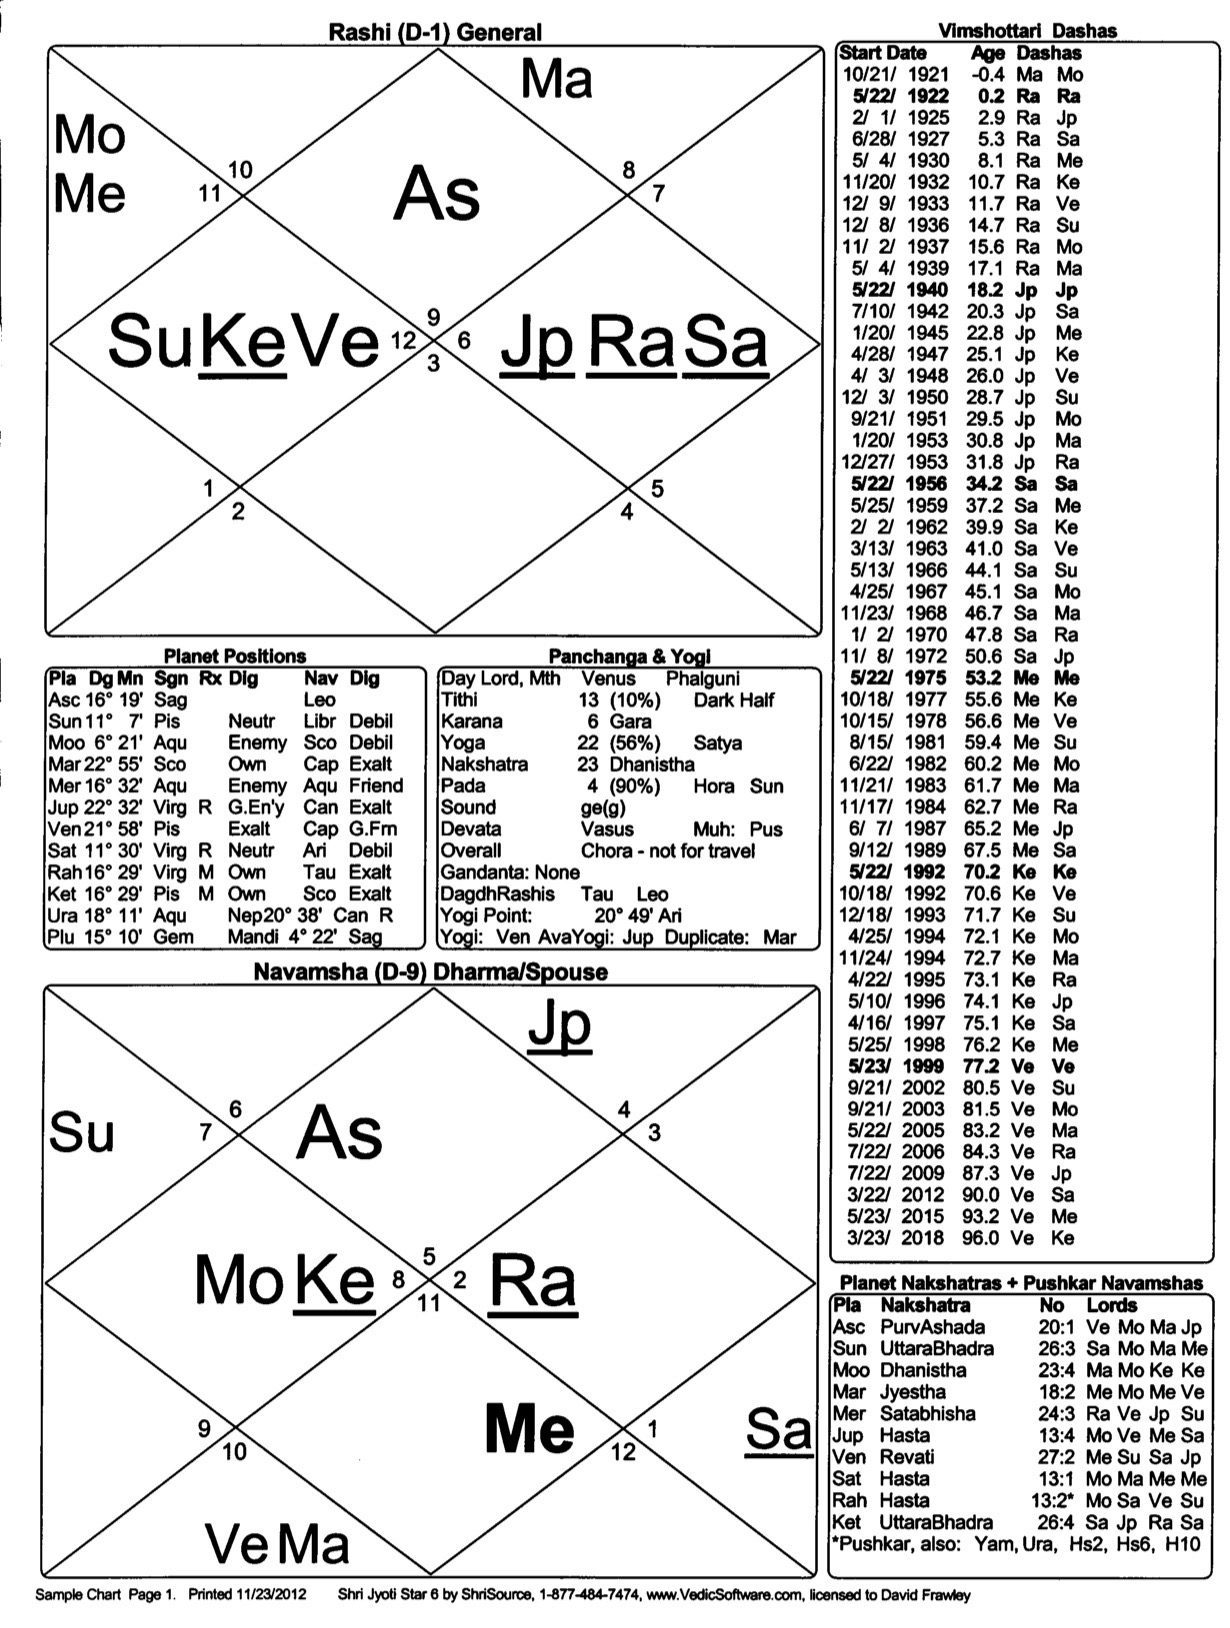
\includegraphics[width=10cm]{pics/lesson-1-northchart1.jpg}
\caption{}
\end{figure}


Note the angular (1 , 4, 7, 10), succedent (2, 5, 8, 11) and cadent houses (3, 6, 9, 12). These are all evident and easy to read from the chart. Mark them with different colors to make them more clear if you wish.

 

Now look at other house configurations. Note the position of dharma (1, 5, 9), artha (2, 6, 10), kama (3, 7, 11) and moksha (4, 8, 12) houses. These will be the same in all North Indian charts.

Then note all apachaya (2, 4, 7, 8) and upachaya houses (3, 6, 10, 11). Though these do not follow a recognizable pattern they will always fall in the same place in the chart.

 

Now look at thesample chart. The number 9 indicates the sign Sagittarius, the ninth sign as the Lagna. The number 10 is Capricorn, 11 is Aquarius and so on around the zodiac.

 

Now look at the specific positions of the planets. You will see an evident grouping of planets in both the fourth and tenth houses, two of the four angles. Note that both natural benefics like Venus and Jupiter, and natural malefics like the Sun, Saturn and Rahu-Ketu, are involved. Since both malefics and benefics are found, the results of the chart are bound to be mixed.

However a malefic influence is predominant, with more malefic planets involved, showing more difficulties than ease in life. The Sun, Saturn, and the Rahu-Ketu axis are natural malefics. Of these planets only the Sun is also a temporal benefic as the ninth house ruler. Venus is not a temporal benefic for Sagittarius Ascendant, ruling the sixth and eleventh houses. Jupiter, though a great benefic and Ascendant lord, being retrograde becomes unpredictable and gives mixed results.

 

The other natural benefics, Mercury and the Moon, are in the third house, which is not a good house for them, though is not in itself very bad. The Moon moreover has some malefic status as the lord of the eighth house, Cancer. In addition it is waning and close to the Sun and becomes malefic on this account. It is also in the sign of a malefic, Saturn. Mercury is a temporal malefic for Sagittarius, ruling the seventh and the tenth (therefore blemished as a benefic by its lordship of two angular houses). The combination of Mercury and the Moon, the planet of the intellect and that of the emotional nature, is always a point of sensitivity and makes the mind easily disturbed. On top of this is the aspect to these two planets of Mars, another natural malefic. In addition Mercury (Aquarius) and Saturn (Virgo) are in a mutual exchange of signs, bringing more of a malefic Saturnian influence on not only Mercury but the Moon also in Aquarius.

 

Meanwhile Mars, the natural Yoga Karaka for Sagittarius, though positioned in its own sign in the twelfth, is aspected by Saturn, restraining and weakening it. A weak Kala Sarpa Yoga (all the planets between the lunar nodes) also exists because Venus is slightly beyond Ketu and Saturn slightly before Rahu.

 

Hence a simple examination of house positions in this chart following a few simple rules shows many inherent difficulties, with some saving grace from Venus and Jupiter. This is a good way to start looking into a chart. Dont worry about the details of particular houses or domains of life at first but first establish the general strength or weakness of the chart. Once this is done you have the foundation to look at specific factors with precision.

 

In the particular chart, the native has had a mixed career with many rises and falls under the Jupiter-Saturn-Rahu tenth house influence. This combination in the tenth house in an Earth sign makes him a businessman, but ambivalent about his career. He has a curious and creative but sometimes unstable mind, with the Mercury-Moon complications. We see an intellectual-artistic person compelled to function as a business and family man with mixed results in all fields. The person is basically out of place in life. Unfortunately there was no one to help the person when they were young to create a more appropriate life-style for him.

 

The dominance of Saturn in the tenth house is particularly difficult. It aspects Venus, the seventh house and its lord Mercury (by mutual exchange) harming the affairs of the seventh house, and causing the native to divorce. It aspects the tenth house and its lord, thus bringing instability in the career. Generally when Saturn is so dominant a negative karma keeps a person from doing what they want or being themselves.

 

But let us not get to focused on the interpretation of this chart, the main example here I want to point out here is planets in angles and how both benefic and malefic planets will give mixed results in such a combination.

 

\subsubsection{The North Indian Moon Chart}

 

Viewing the Chandra or Moon chart you can see how the angles from the Moon are dominated by Mars in the tenth, disturbing the Moon-Mercury combination. Mars in its own sign in the tenth gives some initiative and success, but this has a disturbing effect upon the mind, and is limited by the influence of Saturn.

 

Venus exalted in the second from the Moon as the Yoga Karaka from Aquarius should give good income but malefic aspects to it reduce its consistency. The lord of the Moon, Saturn, afflicted in the eighth house, is another weakening factor, and exchanges signs with Mercury in the Moon sign. But again just learn to look at patterns at first, dont worry about the details of interpretation.

 

Discussion of the Houses in North Indian Chart
 

Using the help of the North Indian chart let us reexamine the basic issues of house interpretation. Houses are divided up in various ways, as we have already noted in our study. Here we will summarize the main factors of house categorization and add some additional points clarity. Study these house positions from the North Indian chart to help you to familiarize yourself not only with them but with the North Indian Chart.

 

\subsubsubsection{Angular Houses}

 

Angular houses – 1, 4, 7, 10 – are places of strength. They are houses of fortune or Lakshmi Sthanas, places of the Goddess. The first house indicates our own bodily health, personal well being and character. The fourth indicates our emotional happiness and our home. The seventh indicates our partner and our marriage happiness. The tenth indicates our career and public success. These are the four main sources of human happiness. Benefics here increase these factors of happiness while malefics decrease them. The same is true of benefic or malefic aspects to these places.

 

Malefic planets like Mars and Saturn with their angular fourth and tenth aspects are particularly difficult located in angles. Similarly benefics in angles to one another tend to strengthen each other, while malefics in angles to other malefics or to benefics tend to cause harm.

 

\subsubsubsection{Trine Houses}

 

Trine houses – 1, 5,  9 – are places of principles and values and all relate to Dharma. They are houses of God or Vishnu (Vishnu Sthanas). The first shows the principles of our personal life, our svadharma or natural duty. The fifth indicates our children or family duties on one level, but on a higher level shows our creative and intellectual principles. The ninth shows our education and our spiritual and religious values, Dharma in the highest sense. Benefics are helpful in trines and malefics are harmful, just as in angular houses. Naturally, Jupiter with its trine aspect is the best planet to have in trines and spread its influence too all three. Benefics in mutual trines to each other gain more strength, while malefics in mutual trines cause more harm.

 

\subsubsubsection{Raja Yoga}

 

What is most sought after is a union of Vishnu and Lakshmi or Trine and angular houses and their lords. This creates a Raja Yoga or royal union that unites our values with fortune and brings great success in life. This can be achieved in some Ascendants through one planet that rules both houses, like Mars for Cancer Ascendent ruling the fifth and tenth houses, an angle and a trine. It can also be achieved by mutual aspects or by exchange of signs between the lord of an angle and the lord of a trine. It is strongest if an angular and trinal lord exchange these houses. For example, for Gemini Ascendant if Jupiter, the tenth lord, is in Aquarius, the ninth house, and Saturn, the ninth lord, is in Pisces, the tenth house, this Yoga is very strong.

 

\subsubsubsection{Duhsthanas}

 

Houses 2, 6, 8 and 12 generally cause difficulties, particularly 6, 8 and 12, the well known Duhsthanas or bad places. The second, though not as difficult as the other two, is a maraka house and can cause harm.  Look at the North Indian chart and you can see how these houses surround either the first or seventh houses. That is they can inhibit either the first house or the seventh house. They represent the transitional points or twilight before and after sunrise and sunset indicated by the first and seventh houses, which are times of instability.

 

Generally all planets suffer in these houses, with the exceptions of malefics in the sixth and benefics in the second, which nevertheless can still have their complications. These four positions can be contrasted with 1, 4, 7 and 10, which are positions of strength. Any planets in 2-12 or 6-8 relationships from one another are likely to have complications, particularly in their mutual periods.

 

\subsubsubsection{Upachaya and Apachaya Houses}

 

Upachaya houses – 3, 6, 10, 11 – follow no particular mathematical pattern. Malefics do well in these positions, except the tenth where only the Sun is generally good and the others only become good if located in their own sign or exaltation. Benefics do well in the tenth and eleventh but suffer in the sixth, and, to a lesser degree, in the third. Of these upachaya houses, the third and eleventh are the houses of brothers, sisters and friends. Hence any signs or planets in 3-11 are usually helpful to one another.

 

Similarly Apachaya houses – 2, 4, 7, 8 – follow no particular pattern either. Malefics cause trouble in these positions as these are important houses of wealth, happiness and longevity. Benefics are good in the first two of these houses. In the seventh even benefics can cause complications and in the eighth are weakened as well.

 

\subsection{The South Indian Chart and Examination of the Signs}
 

The South Indian chart is what I would call a “sign chart” because in it the signs are constant.

 

This chart can be hard to read at first because in it the signs are usually not named or numbered. As Pisces marks the upper left and the other signs are counted off from it in a clockwise direction there is no need for such a marking once one knows the system. The first house is marked by a diagonal line made across it or by LG or ASC, short for Lagna or Ascendant, written in it. The reason for this is once the Ascendant is marked the position of the other houses is obvious.

 

However modern software programs do allow us to place the sign names and house numbers in the South Indian chart, which we should always do for our clients when we give them their charts, as they will not know the intricacies of how the chart is read.

 

The advantage of the South Indian chart is that sign positions, particularly yogas and aspects are more clear. Once the Ascendant is indicated the house rulerships of all the other planets can be clearly seen by the position of the signs that they rule.

 

For learning sign positions, sign qualities, sign rulership, and places of exaltation this chart is easier to use. Similarly for examining the house lords from different Ascendants this chart is also better.

 

One does not need to construct a Moon chart for it but can simply read the planetary positions from the Moon as the Ascendant. The same is true of the Sun, other planets, or other houses.

 

Look at our sample chart using the South Indian chart. First of all you will notice that the house positions are not so obvious. They do not jump out at you or stare you in the face as they do in the North Indian chart. On the other hand, sign positions dominate the chart.

 

Yet the numbers of the houses has been provided for you as AS ascendant will always be 1 or the first house, with the next sign clockwise from it being house 2, and so on around the zodiac.


\subsubsection{Sample South Indian Chart}

 \begin{figure}[h]
\centering
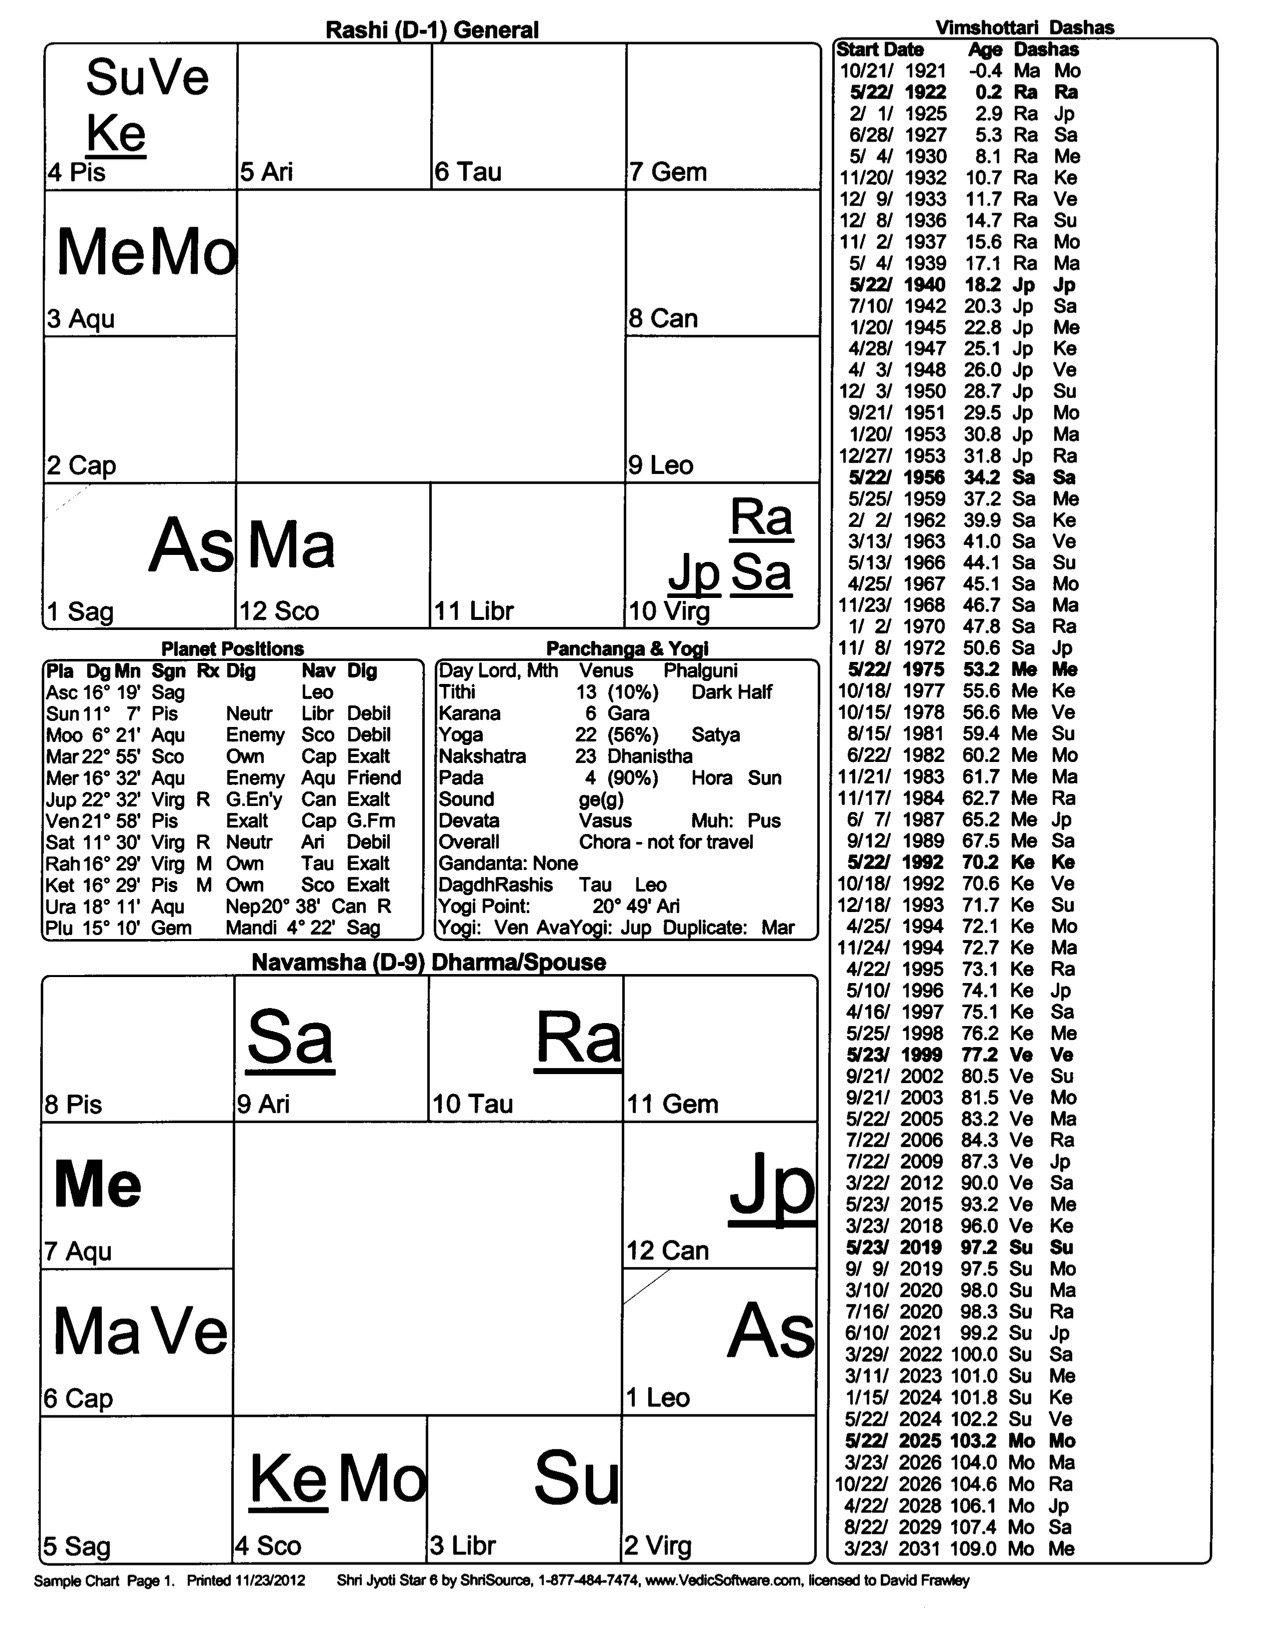
\includegraphics[width=10cm]{pics/Lesson-1-southchart2.jpg}
\caption{}
\end{figure}


 

\subsubsubsection{Referred Houses}

 

The South Indian chart is of particularly advantage in viewing “referred houses,” which occurs when we read different houses as the Ascendant for examining different aspects of the chart.

 

Take the fourth house in the sample chart, the house of the mother and read planetary positions from it as if the Ascendant were Pisces. You can see at a glance that the Sun, Venus and Ketu will be in the house of the mother, while Jupiter, Saturn and Rahu are seventh from it.

 

Take the fifth house, the house of children, and do so as well, as if the Ascendant were Aries. It is immediately evident that the Sun, Venus and Ketu are twelfth from it, while Jupiter, Saturn and Rahu occupy the eighth.

 

Do the same with the third house, the house of brothers and sisters, the seventh, the house of the partner, and the ninth, the house of the father.

 

The South Indian chart is a “movable chart dial in terms of houses” that can be turned quickly to reveal all these changing positions. While the same positions can be read from the North Indian chart, it requires much more difficulty to do so. Generally a separate chart will have to be drawn for each.

 

The North Indian chart helps us understand the houses and their importance. The South Indian chart helps us understand the signs and referred house systems. Each chart therefore helps us look at the astrological positions in a different way. That is why it can be good to look at each chart. However, most astrologers prefer one chart over the other. In this regard, I prefer the South Indian chart.

